\documentclass[a4paper]{article}
\usepackage[spanish]{babel}
\usepackage[utf8]{inputenc}
\usepackage{caratula}
\usepackage{graphicx}
\usepackage{color}
\usepackage{listings}

\usepackage{amsmath}
\usepackage{amsfonts}
\usepackage{multicol}

\textwidth 160mm
\topmargin 0mm
\oddsidemargin 0mm

\usepackage{manycolors}
\usepackage{m2codecolor}

\DeclareGraphicsExtensions{.pdf,.png,.jpg}

\materia{Programación de Sistemas Operativos}
\titulo{Trabajo Pr\'actico 1}
\subtitulo{Desarrollo de un Kernel básico}

\integrante{Alejandro Mataloni}{597/07}{amataloni@gmail.com}
\integrante{Emiliano Mancuso}{706/07}{emiliano.mancuso@gmail.com}
\integrante{Martin Miguel}{181/09}{m2.march@gmail.com}

\lstset{language=[m2]C}

\newcommand{\file}[1]{\textit{#1}}
\newcommand{\func}[1]{\lstinline{#1}}

\begin{document}

\maketitle
\tableofcontents
\newpage

\section{Introducción}
El presente trabajo práctico comienza con el desarrollo de un sistema operativo. Este práctico conforma una parte de una serie de trabajos. El acumulado de estos trabajos llevaran a la consolidación de un kernel pequeño pero funcional. El objetivo de esta primera entrega es crear las unidades básicas de funcionamiento del kernel que sirvan como cimientos para los próximos avances. Entre estas unidades básicas se encuentran: 

\begin{itemize}
  \item una biblioteca para el manejo de la pantalla
  \item un sistema de debug basado en interrupciones
  \item un módulo encargado del manejo de la memoria mediante paginación
  \item un módulo capaz de cargar y descargar tareas del procesador así como manejar colas de espera entre ellas
  \item un módulo que implemente un algoritmo de scheduling para manejar el orden en que se ejecutarán las tareas en el procesador y la implementación de semáforos para operaciones de kernel
\end{itemize}

La red conformada por la relación de todos estos sistemas serán luego la base para la construcción de nuevas estructuras y funcionalidades en el kernel en los próximos trabajo prácticos. 

\newpage
\chapter{Primera versión}

\section{Módulos}

En esta sección se explica la funcionalidad exportada de cada uno de los módulos desarrollados, así como detalles de implementación importantes para comprender el funcionamiento del módulo o para cuidados necesarios en su uso o futuros desarrollos. 

% A continuación se presenta la estructura de archivos fuentes del proyecto.

% \begin{multicols}{2}
% \begin{verbatim}
%  pso
%   \--src
%       |-- bin -- *
%       |-- boot -- *
%       |-- include
%       |   |-- bios.mac
%       |   |-- debug.h
%       |   |-- errors.h
%       |   |-- gdt.h
%       |   |-- i386.h
%       |   |-- idt.h
%       |   |-- isr-def.mac
%       |   |-- isr.h
%       |   |-- klib_machine.h
%       |   |-- lib_str.h
%       |   |-- loader.h
%       |   |-- mm.h
%       |   |-- pic.h
%       |   |-- pso_file.h
%       |   |-- sched.h
%       |   |-- sem.h
%       |   |-- syscalls.h
%       |   |-- tasks.h
%       |   |-- tipos.h
%       |   |-- tss.h
%       |   '-- vga.h
%       |-- kernel
%       |   |-- a20.asm
%       |   |-- debug.c
%       |   |-- gdt.c
%       |   |-- idt.c
%       |   |-- interrupt.mac
%       |   |-- isr.asm
%       |   |-- kernel.c
%       |   |-- kinit.asm
%       |   |-- klib_machine.c
%       |   |-- lib_str.c
%       |   |-- loader.c
%       |   |-- mm.c
%       |   |-- pic.c
%       |   |-- sched.c
%       |   |-- sem.c
%       |   |-- syscalls.asm
%       |   |-- tasks.asm
%       |   |-- tss.c
%       |   \-- vga.c
%       |-- Makefile
%       |-- tasks
%       |   |-- pso_head.asm
%       |   |-- pso_tail.asm
%       |   '-- task1.c
%       \-- tests
% 	  |-- bit_check-test.c
% 	  |-- Makefile
% 	  \-- num_into_string-test.c
% \end{verbatim}
% \end{multicols}

\subsection{Inicialización del kernel}

Este módulo se conforma por dos archivos encargados de toda la inicialización del kernel. El principio de la ejecución de nuestro código sucede en \file{kinit.asm}, que activa la línea a20 y pasa a modo protegido. Para ello utiliza la gdt estática declarada en \file{gdt.c}. Esto luego desemboca en la función \func{kernel\_init()}. Esta función es la encargada de llamar a los inicializadores de los módulos de forma que todos los aparatos del kernel estén listos para trabajar.

\subsection{GDT}

El módulo GDT, conformado por los archivos \file{gdt.c} y \file{gdt.h}, es la definición en C de la gdt. En esta se definen estáticamente los 4 segmentos flat de código y de datos, dos para anillo 0 y dos para anillo 3. Además se define una entrada para la única TSS que utilizamos. Esta debe definirse dinámicamente y lo hace la función \func{gdt\_init()}. Esta GDT representa un modelo de segmentación flat, la forma de eludir el sistema de segmentación del procesador. La idea detrás de esto es usar el sistema de paginación para el manejo estructurado de la memoria física y como mecanismo de memoria virtual. 

\subsection{VGA}

Este es el módulo que provee la funcionalidad para el acceso a la pantalla. En esta etapa la pantalla solo se accede en modo texto, escribiendo caracteres es un espacio de 25 filas por 80 columnas, a 2 bytes por celda. Para trabajar en la pantalla se utilizan 3 funciones: \func{vga\_write(...)}, \func{vga\_printf(...)} y \func{printf(...)}. La primera permite escribir un string en algún lugar de la pantalla especificando fila, columna y formato del texto. La segunda permite escribir un string formateado definiendo también posición en pantalla y color del mismo. Un string formateado es un string que declara internamente lugares que son rellenados con el valor en string de la variable. Esto lo hace de forma análoga al string \emph{fmt} de la función \emph{printf()} de la biblioteca standard de C, aunque con funcionalidades limitadas. Para hacer esto se basa en una biblioteca creada para este sistema, \file{lib\_str.c}, que contiene funciones necesarias para la generación del string final. Por último, la función \func{printf(...)}, hace una réplica más fuerte a la función de C ya que trata a la pantalla como una consola. Esta función imprime al principio de la siguiente fila que ya fue escrita por la función, y de llegar al final de la pantalla mueve todo lo escrito una fila hacia arriba. Para mantener la fila actual se usa una variable global que solo es modificada por esta función. Esta función resultó sumamente útil para imprimir resultados de funciones de evaluación de nuestros módulos.

\subsection{Interrupciones}

Para trabajar con interrupciones se armaron los siguientes 3 archivos con distintas funciones relacionadas: \file{idt.c}, \file{isr.asm} y \file{interrupt.mac}. En \file{idt.c} está declarada la idt propiamente dicha y se cuenta con \func{idt\_init()}, lugar para inicializaciones varias relacionadas a la idt, y \func{idt\_register(...)} que permite registrar una función como respuesta a un número de interrupción dado. La \func{idt\_init()} además remapea los PICs a la posiciones 0x20 y 0x28, de forma que las interrupciones de el mismo sean consecutivas a las del procesador. Para ello usamos \func{pic\_reset(...)} y \func{pic\_enable()}) del archivo \file{pic.c}. 

Por distintos motivos, es necesario que las funciones que son accedidas mediante una interrupción estén en assembler. Estas definiciones se encuentran en distintos archivos .asm. En particular \file{isr.asm} es un lugar para declarar rutinas de atención a interrupción varias. Este archivo funciona que conjunto con \file{interrupt.mac}, donde están declarados varios macros que facilitan el trabajo. El macro \func{isr\_define\_ep} sirve para declarar una isr standard que solo llama a una función C, donde no hubo código de error por culpa de la interrupción. El primer parámetro del macro define el nombre de la isr y el segundo la función de C a llamar. El macro \func{isr\_dkp\_e} sirve para definir una isr que llama a \func{debug\_kernelpanic} (ver módulo Debug). Recibe como parámetros una etiqueta para la isr y un número de interrupción. La otra versión del macro, \func{isr\_dkp\_E} es idéntica a la misma pero asume que el procesador dejó en la pila un código de error y se encarga de trabajarla bajo esas condiciones. Estos macros se encargan de preparar en pila los parámetros para llamar a \func{debug\_kernelpanic(...)}.

\subsection{Debug}

En este nivel de trabajo, nuestra mayor herramienta de debug (además de las provistas por la máquina virtual) son las mismas interrupciones del procesador. El objetivo del módulo de debug es tratar de salvaguardar alguna información del estado de la máquina cuando se produce una de estas interrupciones. La función \func{debug\_kernelpanic(...)} recibe información del estado de la pc (valor de distintos registros de propósito general y de control) al momento del la interrupción inesperada y la imprime en formato de una pantalla de \emph{kernel panic}. La función \func{debug\_init()} registra todas las interrupciones a la función de impresión utilizando los macros \func{isr\_dkp\_*} en \file{interrupt.mac}. En debug también se declara y registra en idt una función particular para la interrupción del timer tick de forma que esta no frene el funcionamiento de la pc. La función (\func{isr\_timerTick\_c}) imprime un relojito en la esquina inferior derecha de la pantalla para mostrar que el mismo está interrumpiendo. 

\subsection{Memory Management}

El manejo de la memoria física y virtual se hace utilizando los sistemas de paginación del procesador. \file{mm.c} contiene todos los métodos para trabajar con estos sistemas. Internamente es necesario mantener información sobre los marcos de páginas. Considerando que se utilizan separadamente algunos marcos para kernel y otros para usuario, estos se tratan de forma se parada. El sistema de directorios del procesador contiene numerosa información sobre el uso de las páginas, en su sentido virtual, es por esto que nosotros debemos guardar aparte información sobre los marcos de página. En particular nos interesa saber cuales están libres y cuales no. La estructura utilizada para guardar esta información es un arreglo de enteros, donde cada bit se corresponde con un marco de pagina. El bit en 1 indica que la página está ocupada, en 0 que está libre. Estas estructuras se acceden mediante las funciones \func{void* mm\_mem\_alloc()}, \func{void* mm\_mem\_kalloc()} y \func{void mm\_mem\_free(void* page)}. A fines de mantener modularidad, estas funciones trabajan solo con las estructuras de marcos de página, y no con las tablas de páginas y directorios. Para lograr verdaderos efectos en el sistema de paginación estas funciones deben utilizarse en conjunto con otras.

Para trabajar particularmente con un directorio de páginas se desarrollaron las funciones \func{mm\_page\_map}, \func{mm\_page\_free}, \func{mm\_dir\_free}, \func{mm\_table\_free} y \func{mm\_dir\_unmap}. Todas estas funciones reciben o devuelven direcciones a distintas secciones del sistema de directorios y se encargan de mapear y desmapear direcciones virtuales a reales en estas estructuras. A excepción de \func{mm\_dir\_new} y \func{mm\_dir_free}, estas funciones no se preocupan si las páginas físicas a las que se están refiriendo están ocupadas o no, o si están marcadas como ocupadas en nuestras propias estructuras. Es responsabilidad de quién las utilice de asegurarse que las direcciones provistas sean correctas. \func{mm\_dir\_new} y \func{mm\_dir\_free} son funciones más autocontenidas que arman y desarman directorios de páginas, pidiendo y devolviendo nuevos marcos de páginas. \func{mm\_page\_map} también pide marcos al kernel si requiere una nueva página para una tabla de páginas. 

Las estructuras del \textbf{mm} se inicializan con la función \func{mm\_init()}. Esta función llena de 0s la estructuras que mantienen la información de los marcos de páginas. En este sistema se asume que contamos con al menos 4mb de memoria ram, ya que se asume que el mapa de memoria física para procesos de usuario empieza luego de eso y necesitamos memoria de usuario. De esta forma, la cantidad de marcos de páginas de kernel es fija. En cambio, dado que cuanta memoria tiene el sistema no es un valor constante, el proceso de inicialización debe contabilizar la cantidad de memoria disponible y guardar esta información. Esto se realiza con el método \func{uint\_32* memory\_detect()} y la información se guarda en \func{uint\_32 usr\_pf\_limit} como la cantidad de ints que pueden verificarse en el arreglo que mantiene la información de los marcos de página de usuario. Marcos más allá de ese límite no pueden ser asignados. Para contar memoria se testean secciones de 4kb. La verificación consiste en escribir en la última dirección de la sección y leer. Si el valor es igual al escrito se considera que la dirección es válida y sus 4kb superiores también son memoria accesible. Como solo nos interesa un bloque de memoria contigua, la primera vez que falla la verificación se frena el proceso y la última dirección escrita y leída satisfactoriamente pasa a ser el límite de la memoria útil. 

La inicialización también activa \textbf{PSE}, genera un directorio de paginas básico, actualiza el cr3 y activa paginación. Al activarse paginación, el proceso empieza a utilizar el directorio de páginas apuntado por el cr3 para convertir direcciones virtuales en físicas. Es por esto que el cr3 debe tener un directorio de páginas que posea correctamente mapeada la siguiente instrucción a ejectuar luego de activar paginación. Un criterio general es que todos los directorios deben tener mapeada la memoria de kernel (los primeros 4mb), ya que las estructuras definidas allí deben estar disponibles siempre. Para mapear los 4mb de manera eficiente se utilizan páginas de 4mb permitidas por la función \textbf{PSE} del procesador. En este momento no se está verificando que esta función esté soportada por el procesador, simplemente se asume. Además, por simplicidad, se considera que este primer mapeo es el único de 4mb para cada directorio. 

Finalmente, este módulo posee la función \func{void* sys\_palloc()} que es llamada por la syscall \func{palloc}. Esta syscall es registrada por \func{mm\_init()} como la syscall 0x30, considerando 0x3* el prefijo de las syscalls de memoria. La llamada a sistema permite a una aplicación de usuario pedir una página de memoria y que esta sea mapeada a su espacio de direcciones virtuales. La syscall \func{palloc} devuelve la dirección virtual de la página habilitada para el usuario. 

En \func{mm\_init()} se realizan testeos de todas las funciones nombradas anteriormente. Todas verificaciones imprimen en pantalla. La verificaciones se encuentran comentadas. 

\subsection{Scheduler}
El módulo de scheduler es el algoritmo encargado de decidir cual será la próxima tarea a ejecutarse. Funciona muy relacionado con el módulo \textbf{loader}. El \textbf{scheduler} mantiene un \textit{array} de \func{sched-task}. Ésta estructura contiene el estado y dos enteros (next y prev) que sirven para mantener una cola de tareas sobre un \textit{array}.
En esta cola, sólo mantenemos enlazadas a las tareas que están en estado \textit{RUNNING}.
Además de la cola, el módulo lleva una cuenta del quantum consumido por la tarea actual, el \textbf{pid} de la misma y el indice del ultimo elemento de la cola.

\subsection{Loader}
El módulo del loader se encarga de mantener el \textbf{Process Control block}, cambiar el contexto de las tareas, e interactuar con el \textbf{scheduler}.
Para el \textbf{Process Control block}, creamos una estructura que solo guarda el \func{CR3} y el \func{ESP0} de la tarea, junto con dos indices (prev y next) para armar las colas donde las tareas se bloquearan.
Para administrar los \textbf{pids} tenemos una cola de los libres, así el próximo lo obtenemos en $\mathbb{O}(1)$.
El \textbf{loader} es el módulo que inicializa las tareas, las bloquea, desbloquea y las termina dentro del sistema operativo.
La funcion \func{loader\_switchto(...)} es la encargada de realizar el cambio de tarea. Esta función fue programada en assembler en el archivo \file{loader\_switch.asm} ya que necesita mucho control de bajo nivel como accesos a parte de la TSS, la pila y registros de control como el cr3. En el cambio de tarea es necesario guardar el estado actual de ejecución. El sistema de llamadas a sistema mediante interrupciones y la funciones involucradas en el medio van guardando toda la información importante (exceptuando los valores del \func{CR3} y \func{ESP}) en la pila. Es por este motivo que al cargar una tarea debe inicializarse una pila que responda a estas llamadas. Esto es, cargamos una tarea de forma que parezca que ya estaba corriendo. Como hacemos esto puede verse en la preparación de la pila realizado en \func{loader\_load(...)}. 

Este módulo también define las syscalls \func{getpid} y \func{exit}.


\subsection{Syscalls}

Los archivos \file{syscalls.h} y \file{syscalls.asm} proveen las herramientas para el registro de las llamadas al sistema provistas por el kernel. Las syscalls suelen hacerse mediante interrupciones ya que es un método que nos provee el procesador para cambiar de nivel de privilegio. Nosotros decidimos mantener esta idea y además, para independizarnos de la cantidad de interrupciones posibles en el procesador, las syscalls fueron vectorizadas a dentro de la interrupción \func{0x30}. Esto es, acceder a una syscall particular significa hacer por software la interrupción \func{0x30} teniendo en el registro \func{eax} el número de la syscall a acceder. Este proceso se envuelve en una serie de funciones declaradas en \file{syscalls.h}, cuya verdadera implementación se encuentra en \file{syscalls.asm} y realizan las acciones descriptas anteriormente. La interrupción \func{0x30} está conectada a la isr \func{isr\_syscall} (en \file{isr.asm}), encargada del proceso de vectorización. El vector que relaciona el número de syscall con una función se encuentra en \file{syscalls.h}. Este vector debe ser llenado por la inicialización de los distintos módulos que exporten syscalls en la posición correspondiente con la dirección de la función llamada. 

\subsection{Semáforos de Kernel}

Este módulo permite el manejo de semáforos de kernel. Funciona muy relacionado con el módulo \textbf{loader}. Los semáforos se conforman de dos enteros sin signo. El primero es el valor del semáforo. Si vale 0 significa que hay uno o más tareas esperando el evento del semáforo. Si es mayor a 0 significa que pueden hacerse tantos \func{sem\_wait(...)} como el valor de la variable sin bloquear el proceso. El segundo entero es una cola, y funciona de la misma forma que las colas en \textbf{loader}. La función \func{sem\_wait(...)}, si el valor del semáforo parámetro es 0, encola al proceso actual en la cola del semáforo mediante \func{loader\_enqueue(...)}. La función \func{sem\_signaln(...)} incrementa el valor del semáforo y, si era 0, le avisa al loader que desencole a alguién mediante \func{loader\_unqueue(...)}. La función \func{sem\_broadcast(...)} desencola a todos los miembros de la cola del semáforo y establece su valor en 1, de forma que al menos un proceso pueda pedir el semáforo. 

El módulo no maneja otras estrucutras. Los módulos de kernel son libres de registrar semáforos declarando una nueva variable de tipo \func{sem\_t} e inicializándola con el macro \func{SEM\_NEW(uint\_32 val)}, que asigna al semáforo el valor \func{val} y establece la cola como vacía. 

\chapter{Segunda versión}

\section{Filesystem y dispositivos de almacenamiento}

\begin{figure}[H]
\hspace{-2cm}
% \centering
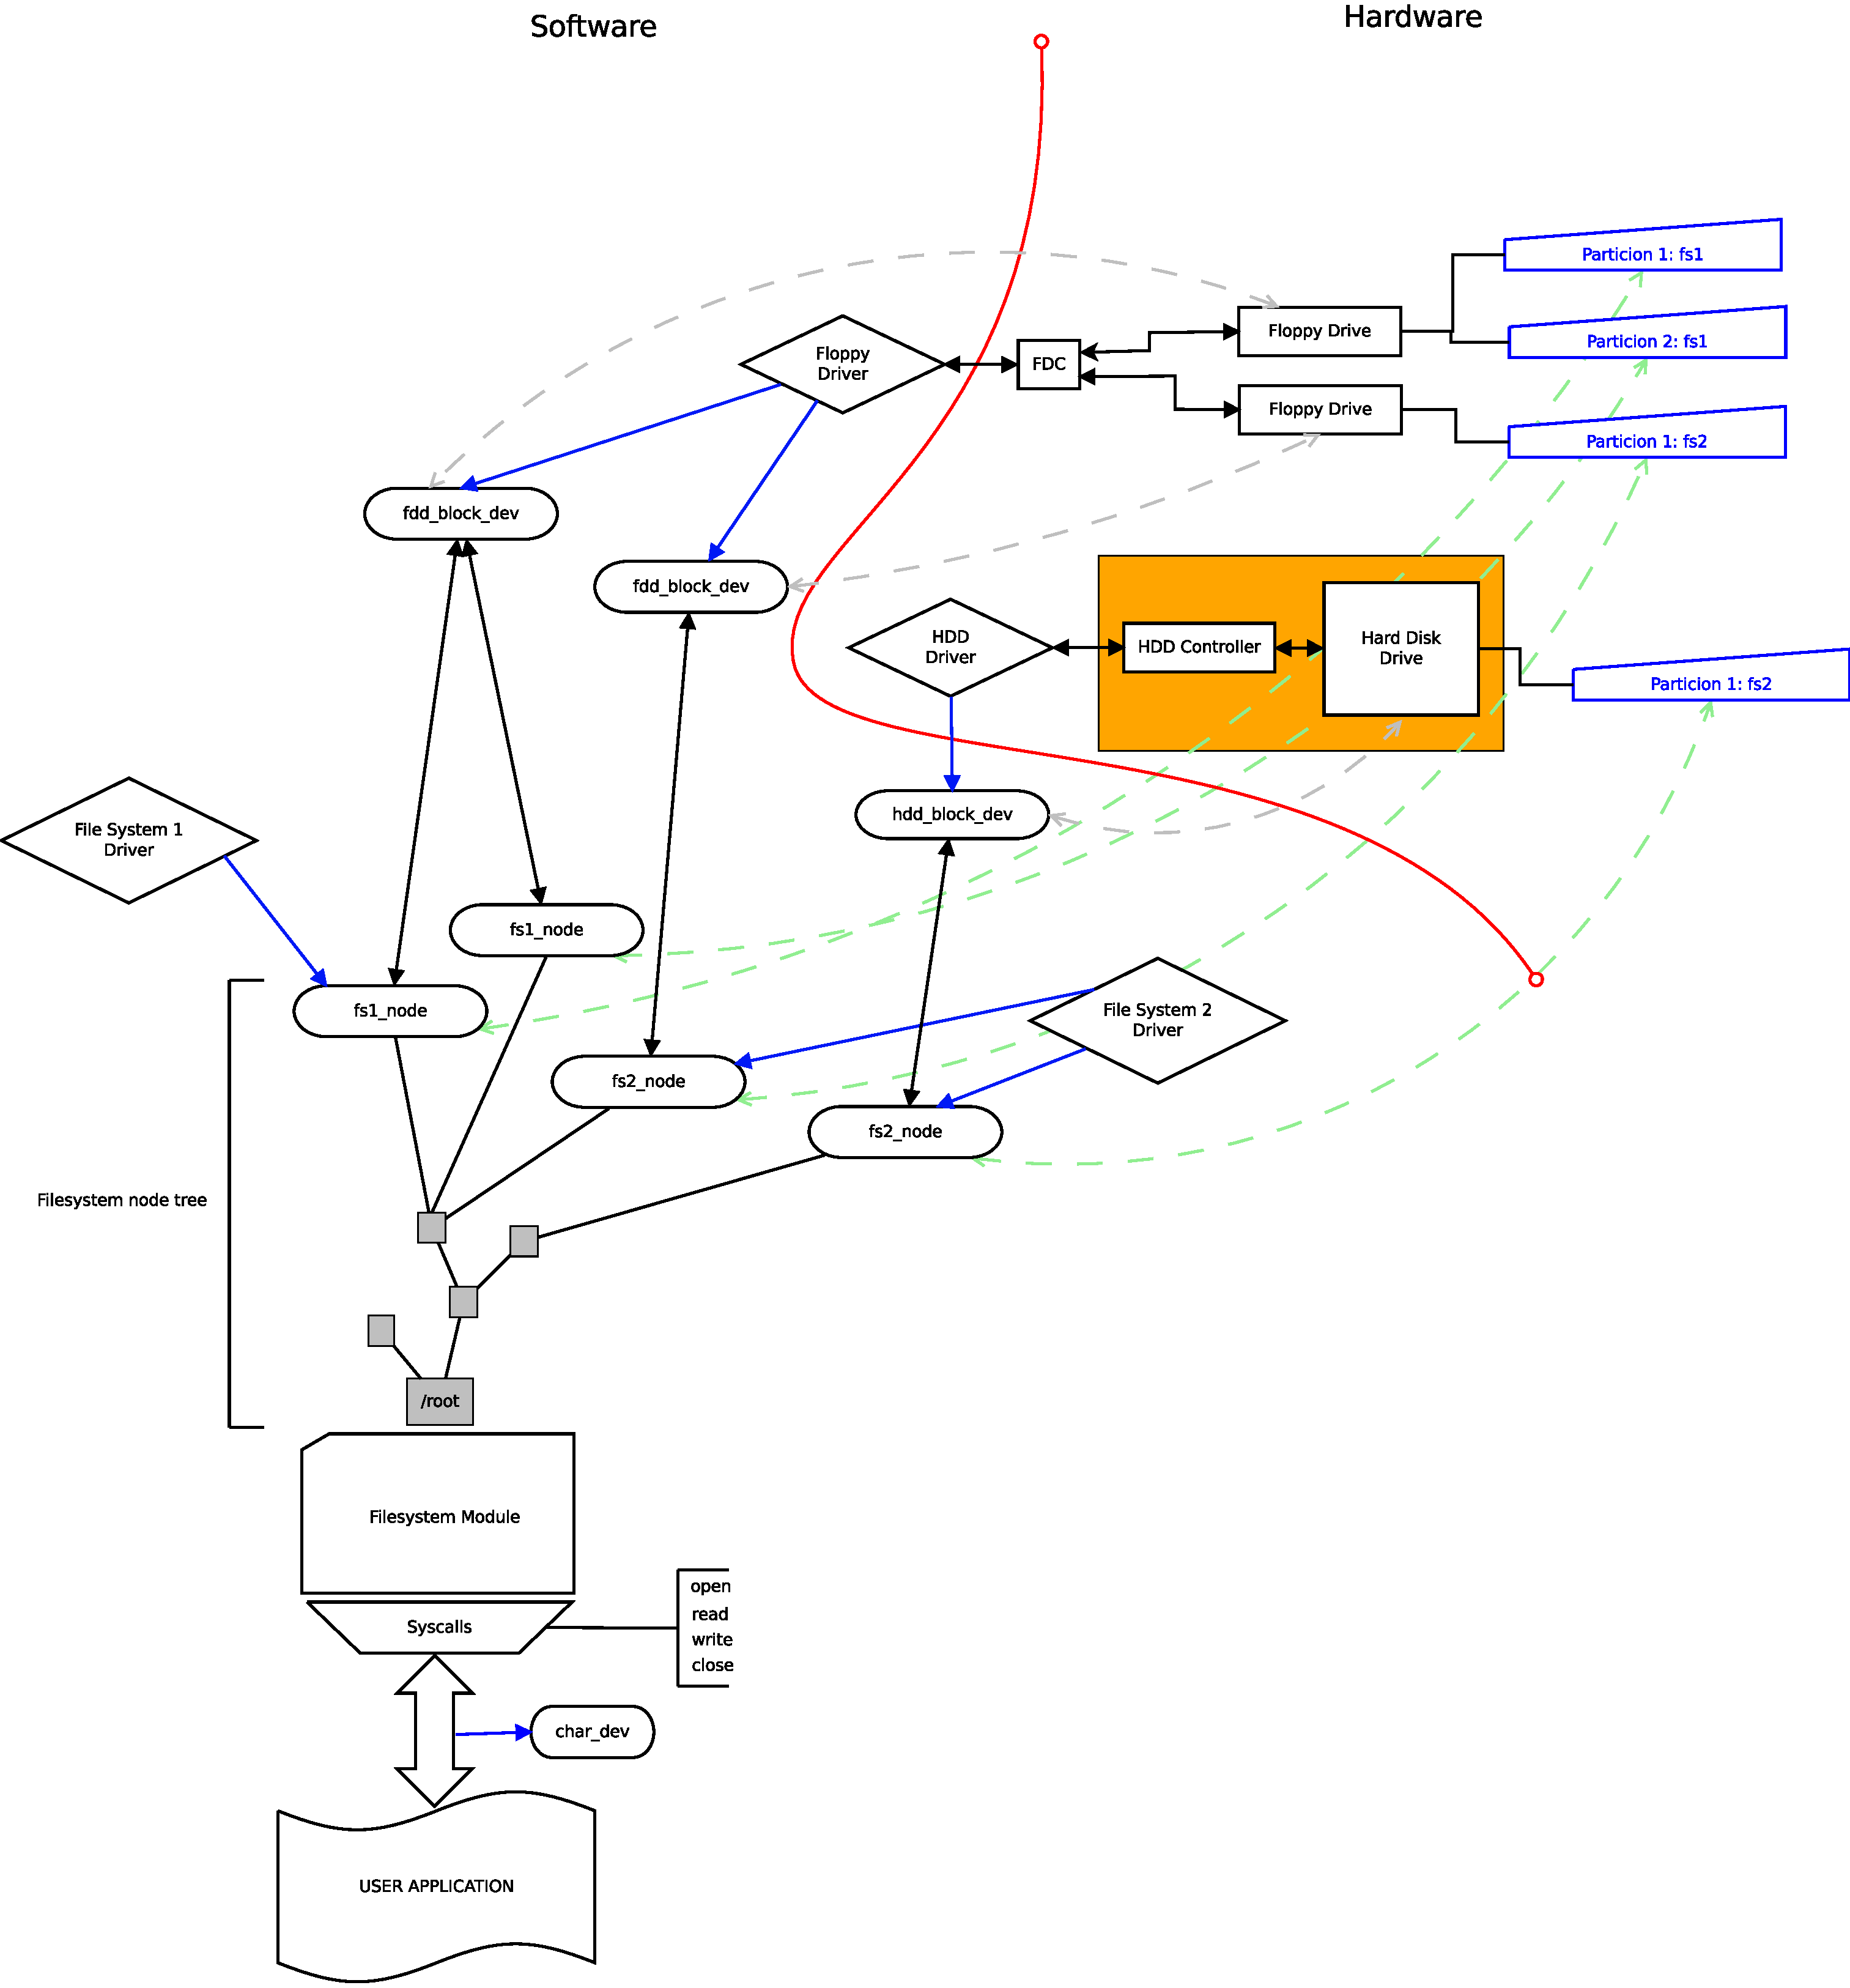
\includegraphics[scale=0.40]{graphics/filesystem-hd.pdf}
\caption{Diagrama de relación entre HW, drivers, devices y el filesystem}
\end{figure}

El gráfico presenta un esquema de relación entre los componentes de Hardware y sus respectivos drivers con el resto del sistema, en particular el módulo de filesystem. Otros elementos de diagrama son nodos y devices, estructuras cuya mayor relevancia se debe a la significancia lógica en el sistema. A continuación se presentan los componentes que hacen a la integración del hardware con el sistema de forma flexible. La principal idea de este esquema es permitir que el sistema se adapte a distintas configuraciones de hardware, manteniendo como primitiva la modularización de las funciones. Esto es, que cada cual se encargue de lo que debe. 

\subsection{Hardware drivers}
Los drivers de hardware son la primera capa de abstracción en software de lo que sucede en el bajo nivel del hardware. En el diagrama, estos serían \func{floppy driver} y \func{hdd driver}. La principal función de estos driver es otorgar una interfaz más amigable al resto del sistema para comunicarse con los dispositivos. Deben tener las funciones necesarias para enviar y recibir mensajes y comandos al dispositivo y manejar errores. Además, debe permitir el uso del dispositivo de forma transparente a las peculiaridades del mismo. Para ello se presentan las estructuras funcionales de \func{devices}. Un \func{device}\footnote{\url{http://en.wikipedia.org/wiki/Device_file}} es una interfaz genérica para la operación con una variedad de componentes. Los \func{devices} se agrupan en tipos, de forma de agrupar los dispositivos por la interfaz con la que pueden trabajarse y así otorgarle al usuario mayor uniformidad a la hora de operar los dispositivos. En particular, los discos de almacenamiento se representan con \func{block devices}. En esta interfaz, se considera que se trabaja con un dispositivos de almacenamiento de datos cuya principal cualidad es la de estar divididos en bloques. La interfaz de un \func{block device} establece que la manera de obtener y enviar información es en formato de bloques, que pueden ser accedidos de forma aleatoria. 

A fines prácticos, entonces, si bien los módulos \func{floppy driver} y \func{hdd driver} poseen numerosas funciones para el trabajo con los dispositivos, en particular exportan \func{block devices}, que a pesar de sus particularidades internas, para el usuario externo todos se trabajan de la misma forma. El \func{block device} presentado por el \func{floppy driver} (\func{fdd\_block\_dev}) es la representación de un único dispositivo de almacenamiento. Esto es, solo puede haber un \func{fdd\_block\_dev} por cada aparato de hardware. En este caso en particular sucede que los muchos dispositivos (varios floppy drives), se agrupan bajo un único controlador (\func{fdc}), que se relaciona con un único módulo de drivers, para luego volver a separarse en \func{devices}. Estos últimos son solo cáscaras del driver y deben mantener la información particular del dispositivo necesaria para utilizar los servicios del driver. Esta información comprende: 

\begin{itemize}
 \item Número de dispositivo 
 \item La geometría del disco en el dispositivo, necesaria para hacer la conversión del número de sector a formato CHS.
 \item Buffer de transferencias. Este buffer (de 512 bytes de tamaño), es necesario ya que la comunicación entre el \func{fdc} y el cpu se hace mediante \func{DMA}, el cuál es solo capaz de acceder el primer MB de memoria física. 
 \item Información de estado del dispositivo. 
 \item \emph{otros...}
\end{itemize}

Por las particularidades del los dispositivos, estos solo pueden ser accedidos uno a la vez. De igual manera, el fdc solo puede ejecutar una operacin a la vez. Esto plantea la necesidad de bloquear los accesos a las funciones formando seccionea críticas. 

\subsection{Filesystem drivers}

\subsection{Filesystem module}



\end{document}
